\documentclass[a4paper,12pt,oneside]{article}
%\documentclass{refart}
\usepackage{graphicx}
\usepackage{listings}
\usepackage[hidelinks=false]{hyperref}
\hypersetup{
	colorlinks   = true, % Color links instead of red boxes
	urlcolor     = blue, % Color for external hyperlinks
	linkcolor    = blue, % Color for internal links
	citecolor    = red % Color for citations
}

% This command modifies the section numbering format, so that the chapter number does not show in the section number. Therefore, since I am not using chapters, instead of having section numbers 0.1, 0.2, etc, I only get sections 1, 2, etc.
%\renewcommand*\thesection{\arabic{section}}

%\setcounter{secnumdepth}{3}

\begin{document}

\title{Matlab Camera Characterization Toolbox v1.0
	   \newline Documentation}
%\subtitle{Documentation}
\author{Victor Medina}

\maketitle

\tableofcontents

\section{Introduction}


%\section{Opening up the main interface}
\section{Main interface}
The Image tools interface can be opened by calling the \textit{Image{\textunderscore}tools} script from the Matlab command line:

\begin{lstlisting}[language=matlab]
>> Image_tools
\end{lstlisting}

This script calls the main user interface for the toolbox, which offers functionality for display and camera characterization, image calibration, and several other utilities. The options available in this menu are (Fig.~\ref{fig:main_menu}):

\begin{itemize}
	\item Calibration tools
		\begin{itemize}
			\item Camera characterization
			\item Display characterization
			\item Image calibration
			\item Image calibration (batch mode)
		\end{itemize}
	
	\item Utilities
		\begin{itemize}
			\item Load image
			\item Select pixels
			\item Delete selection
			\item Average
			\item Colorimetry tests
		\end{itemize}
\end{itemize}

\begin{figure}[h]
    \centering
    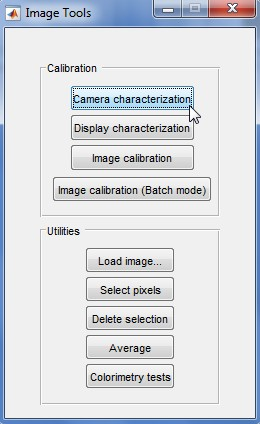
\includegraphics[width=0.5\textwidth]{images/main_gui.jpg}
    \caption{MCCT main menu}
    \label{fig:main_menu}
\end{figure}

\subsection{Camera characterization}

The camera characterization option (Fig.~\ref{fig:camera_characterization_gui}) allows to estimate a camera's transfer function from a series of corresponding colorimetric and radiometric measurements. 

\subsubsection{Characterization process}

This process is meant to be done with some type of color chart (e.g. the Macbeth color chart). The general process consists of the following steps (marked in red in Fig.~\ref{fig:camera_characterization_gui}):

\begin{enumerate}
	\item \textbf{Open a color chart.}
	The \textit{Open color chart} button (Fig.~\ref{fig:camera_characterization_gui}-(1)) allows to load a color chart image (in a new window) to sample the colorimetric values from it. This is typically a photograph of a physical color chart, taken with the same device that we want to characterize under some observation and illumination conditions, with some set of chosen acquisition parameters (focal length, ISO, aperture, and shutter speed).
	
	\item \textbf{Select color pixels and read their value.}
		The \textit{select sample} button (Fig.~\ref{fig:camera_characterization_gui}-(2.1)) creates a pixel selection handle in the color chart window (see Fig.~\ref{fig:color_chart}). This selection handle can be resized and moved around the image with the mouse pointer until it covers all the pixels to be sampled. Once the desired pixels are selected, the \textit{store pixels} button (Fig.~\ref{fig:camera_characterization_gui}-(2.2)) averages their color values (in the original color space of the image) and adds a new entry in the \textit{sampled colors} table (Fig.~\ref{fig:camera_characterization_gui}-(2)).
	\item \textbf{Fill in the radiance table.}
	The radiance values should be measured with some radiance measuring device (in our case, a spectroradiometer) under the same observation and illumination conditions used to photograph the color chart\footnote{Keep in mind that these values will be the same regardless of the acquisition parameters used to photograph each color chart}. These values can be entered in the \textit{Measured radiance} table (Fig.~\ref{fig:camera_characterization_gui}-(3)) either by hand, or pasted from some external file such as an Excel data sheet.
	\item \textbf{Fill in the camera's properties (optional)}
	Optionally, the camera's model and acquisition parameters can be entered (Fig.~\ref{fig:camera_characterization_gui}-(4)) so that they show up in the generated graphs. The main purpose for this option is so that graphs can be distinguished from one another and organized accordingly.
	\item \textbf{Characterize}
	Once all the necessary data has been introduced, the \textit{characterize} button (Fig.~\ref{fig:camera_characterization_gui}-(6)) generates an estimation of both the forward (radiance--\textgreater color) and inverse (color--\textgreater radiance) transform matrices for the device. A correlation vector is computed for each transform matrix, indicating the degree of reliability for each channel's estimation, where 0 is very low and 1 is a perfect correlation. After the estimation process is finished, two plots will pop up (Fig.~\ref{fig:estimated_graphs}) to illustrate the estimated transform function.
\end{enumerate}

\subsubsection[Overexposed and underexposed photographs]{Working with overexposed and underexposed photographs}
In some cases, the illumination and acquisition conditions may result in over- or under-exposed photographs. When this happens, the wrongly-exposed pixels should not be used in the characterization because they may bias the estimation process, producing wrong matrices with a lower correlation. We can automatically exclude these pixels by setting a threshold value for overexposure and/or underexposure (Fig.~\ref{fig:camera_characterization_gui}-(5)). The corresponding radiance entries will automatically be excluded as well to avoid a mismatch between the number of entries in both tables.

\begin{figure}[hp]
	\centering
	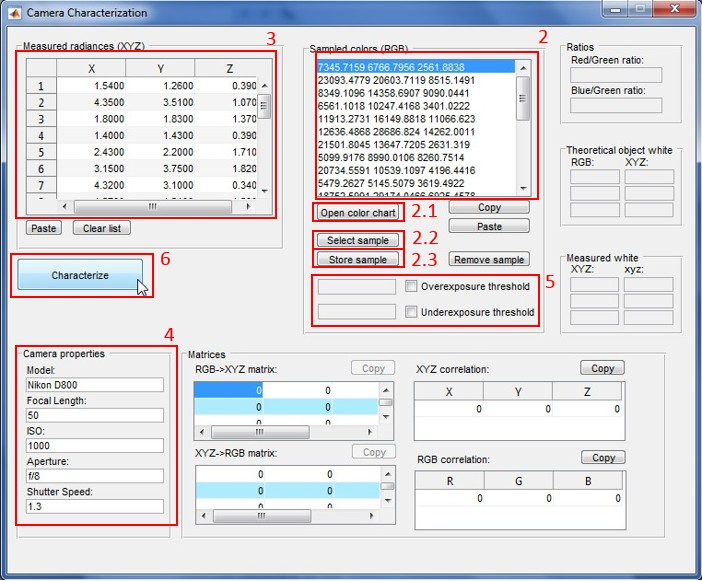
\includegraphics[width=1\textwidth]{images/camera_characterization_gui.jpg}
	\caption{Camera characterization GUI. The numbers in red indicate GUI components referenced in the text.}
	\label{fig:camera_characterization_gui}
\end{figure}

\begin{figure}[hp]
	\centering
	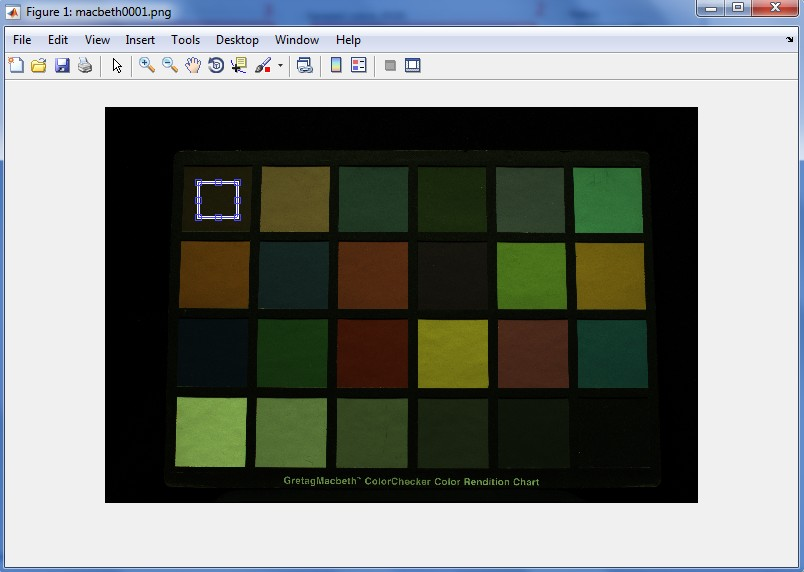
\includegraphics[width=1\textwidth]{images/color_chart.jpg}
	\caption{Macbeth color chart. The selection rectangle in the first color target indicate the pixels that will be sampled.}
	\label{fig:color_chart}
\end{figure}

\begin{figure}[hp]
	\centering
	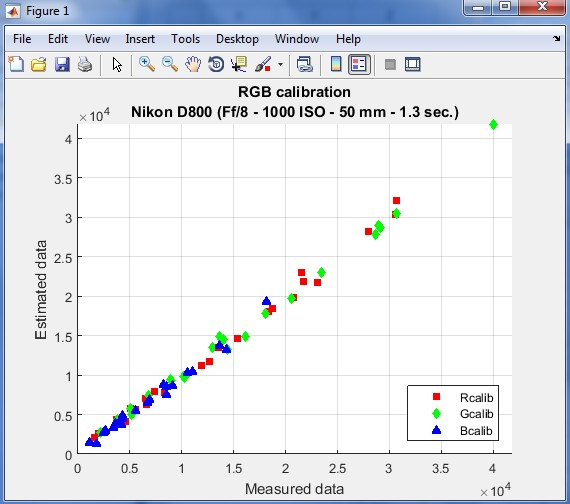
\includegraphics[width=0.49\textwidth]{images/graph1.jpg}
	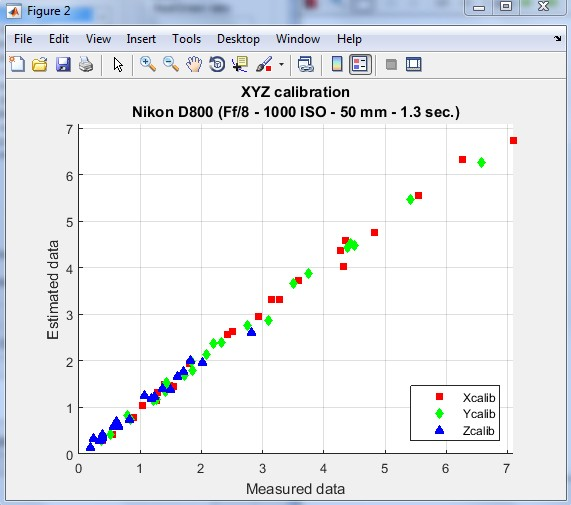
\includegraphics[width=0.49\textwidth]{images/graph2.jpg}
	\caption{Colorimetric (left) and radiometric (right) estimation graphs which show, on the vertical axis, the value calculated with the estimated matrix, for each measured value shown on the horizontal axis. A straight line indicates a good correlation between real and estimated values.}
	\label{fig:estimated_graphs}
\end{figure}

\section{Display characterization}

The display characterization option estimates the color transform function of a display under some observation and illumination conditions, given a set of corresponding colorimetric inputs and measured radiometric outputs ---under those conditions--- and a characterization model. 

\subsubsection{Characterization process}

This characterization process has been optimized for liquid-crystal displays (LCD), but can also be used for other types, such as older cathode ray tube (CRT) displays. Typically, a display is characterized by displaying a set of known monochromatic (i.e. only red-, green-, or blue-channel component) color samples on the screen and measuring the radiance emitted on its surface with some radiance-measuring device (in our case, a spectroradiometer). A model describing the response of the display can then be estimated from the correspondence between input and output.

The process to estimate a characterization model for a display with our tool consists of the following steps (marked in red in Fig.~\ref{fig:display_characterization_gui}):

\begin{enumerate}
	\item \textbf{Fill in the colorimetric input and radiometric output}
	The input color samples and output radiometric measurements must be entered in the corresponding tables (Fig.~\ref{fig:display_characterization_gui}-(1)) for the red, green, and blue samples. Keep in mind that the same number of samples must be entered in all the tables to avoid a mismatch error. 
	\item \textbf{Select the desired characterization model}
	Four models are available to choose from (Fig.~\ref{fig:display_characterization_gui}-(2)): Gain-Offset-Gamma (GOG), Gain-Offset-Gamma-Offset (GOGO), Gain-Gamma-Offset (GGO), and a simple display characterization model based only in one gamma parameter. These four models, traditionally used to characterize CRT displays, are also recommended in the literature for LCD characterization, but since they are often not enough to model some characteristics of LCDs, we use them in combination with an additional transform matrix.
	\item \textbf{Characterize}
	Once all the required information has been filled in, we can proceed with the estimation of the characterization model parameters and the transform matrices (Fig.~\ref{fig:display_characterization_gui}-(3)). The quality of the estimated model is indicated by the coefficient of determination ($R^2$) which represents the goodness of fit, between 0 and 1, with 1 being a perfect fit.
	\item \textbf{Display the characterization graph}
	The \textit{display graph} button (Fig.~\ref{fig:display_characterization_gui}-(4)) opens up a plot that illustrates the correlation between measured and estimated values.
\end{enumerate}

\begin{figure}[hp]
	\centering
	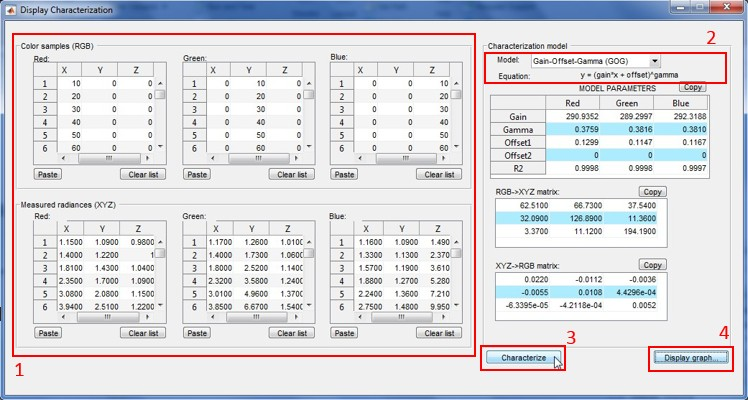
\includegraphics[width=1\textwidth]{images/display_characterization_gui.jpg}
	\caption{Display characterization GUI. The numbers in red indicate GUI components referenced in the text.}
	\label{fig:display_characterization_gui}
\end{figure}

\begin{figure}[hp]
	\centering
	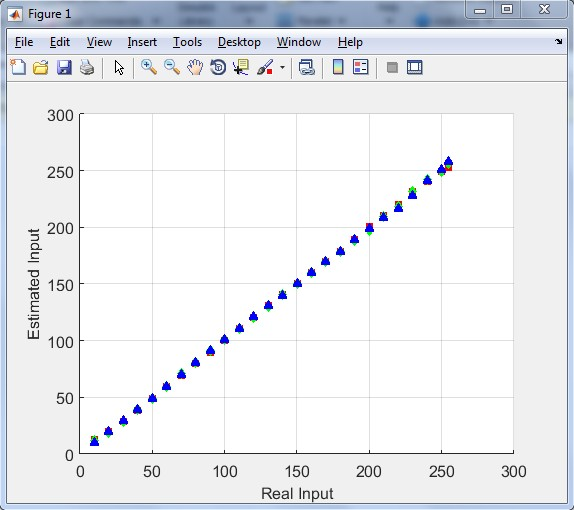
\includegraphics[width=0.6\textwidth]{images/display_graph.jpg}
	\caption{Characterization graph that shows, for a set of measured screen output radiances, the correspondence between real colorimetric input (horizontal axis) and an estimation of the colorimetric input required to produced that same output, using the estimated characterization model (vertical axis). A straight line indicates a good correlation between real and estimated values.}
	\label{fig:display_graph}
\end{figure}

\section{Image calibration}

Image calibration is the process that allows to see how a photograph, taken with a camera whose transform matrix is known, will look on a characterized display. This process is performed in two stages: first, the device-dependent RGB pixel values in the photograph ---which are expressed in the camera's RGB color space (Fig.~\ref{fig:image_calibration_workflow}-(a))--- are transformed into device-independent XYZ pixel values using the camera's inverse transform matrix (Fig.~\ref{fig:image_calibration_workflow}-(b)); then, those XYZ values are transformed back to device-dependent RGB values using the display's characterization model (Fig.~\ref{fig:image_calibration_workflow}-(c))). The result of the first conversion stage gives an approximation of the radiometric information ---in the XYZ color space--- in the scene where the photograph was taken and the second stage produces the final color calibrated image.

The image calibration tool in MCTB provides this functionality as well as the option to export individual channel images from each step of the process. It may be the case that some photographs have a dynamic range higher than that of the display; this tool also offers the option to set a maximum luminance value for a display, as well as a luminance adaptation factor, so that pixel values that fall outside the display's luminance dynamic range can be converted to valid values.

\begin{figure}[hp]
	\centering
	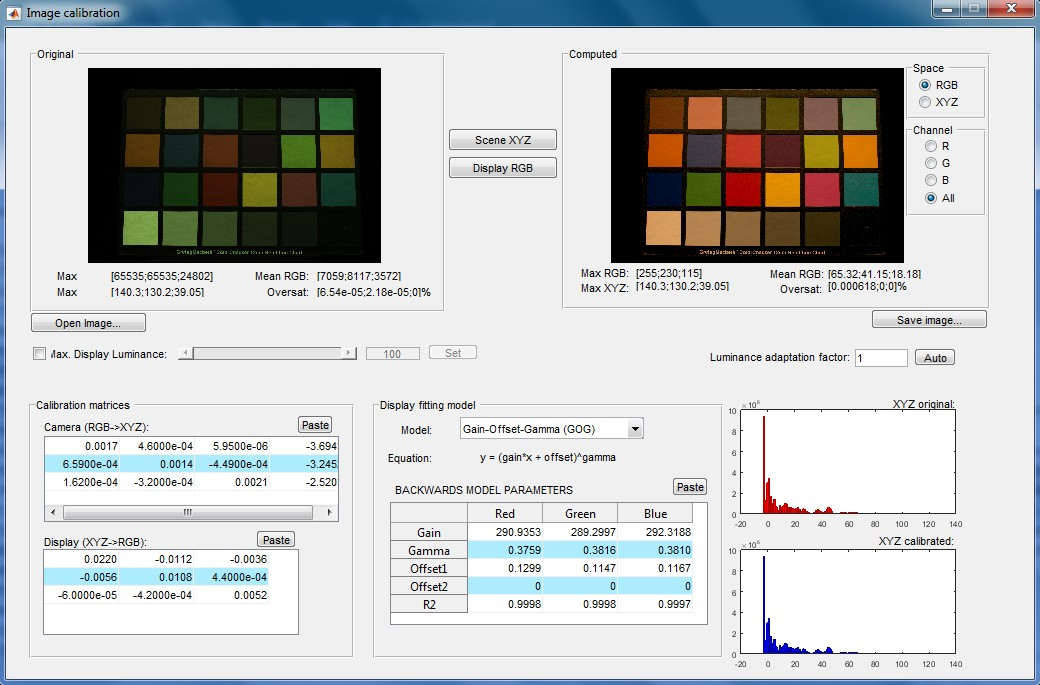
\includegraphics[width=1\textwidth]{images/image_calibration1.jpg}
	\caption{Image calibration GUI.}
	\label{fig:image_calibration_gui}
\end{figure}

\begin{figure}[hp]
	\centering
	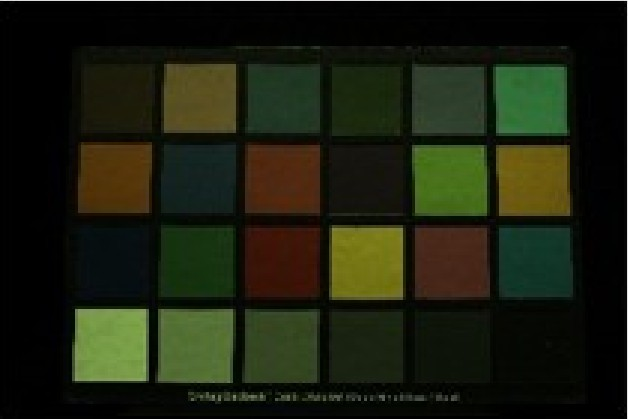
\includegraphics[width=0.32\textwidth]{images/im_calib_step1.jpg}
	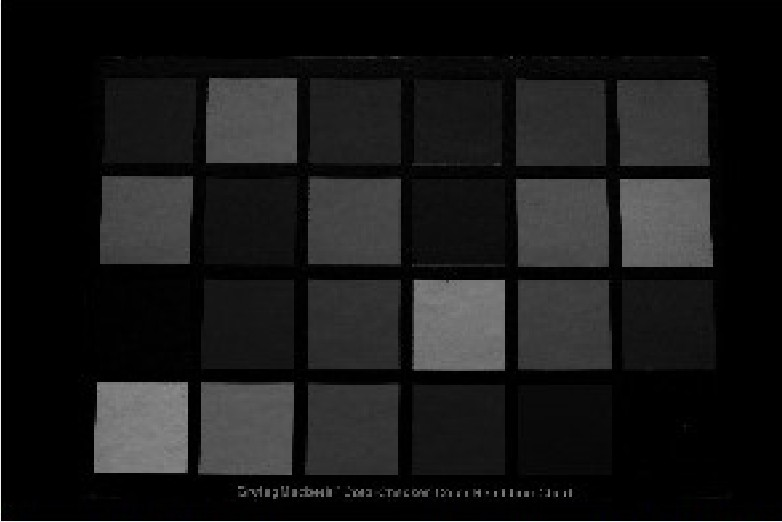
\includegraphics[width=0.32\textwidth]{images/im_calib_step2.jpg}
	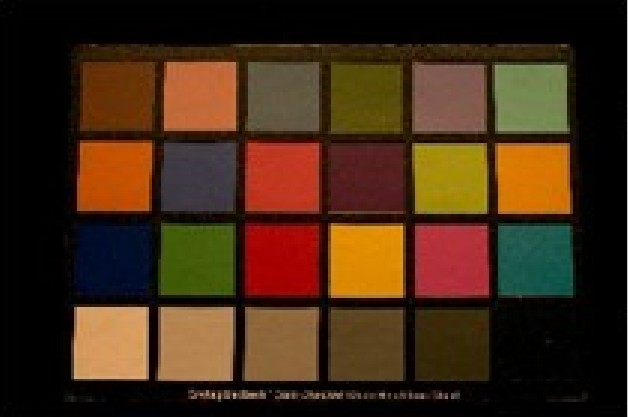
\includegraphics[width=0.32\textwidth]{images/im_calib_step3.jpg}
	\caption{Steps in the image calibration process. From left to right: The original photograph (a) is converted from the camera's RGB color space to a device-independent space (XYZ) (b); then, the image is converted back to RGB using the display's characterization model (c).}
	\label{fig:image_calibration_workflow}
\end{figure}

\section{Image calibration (batch)}

This tool offers a similar functionality as the non-batch version, except that it allows to load several images at once, creating a calibration queue and saving them automatically. This is useful in cases where one needs to calibrate many images for the same camera and display.


\section{Known bugs}
The following is a list of known issues in each version of this software:

Version 1.0:

\begin{itemize}
	\item Common to all:
	\begin{itemize}
		\item 
		Pasting radiance values from an external file throws a button callback error (Error Message: ``Error using reshape'') when numbers use a decimal digit separator other than a point.
	\end{itemize}
	\item Camera characterization:
	\begin{itemize}
		\item 
		Clicking on \textit{select sample} creates a new pixel selection handle every time. While this should not be a big issue, it is worth noting that \textit{store sample} will only sample those pixels selected by the last created handle, ignoring any other existing selection handle.
	\end{itemize}
\end{itemize}


\end{document}